\section{Modeling}
\label{sec:modeling}

This section describe how the best fitting models to predict the Life.expectancy were created. The pre-processed and cleaned dataset contained 157 observations and 23 variables to be considered for the regression model. Three columns: X, Country, and Year, were removed from the pre-processed dataset. Some transformations were applied to produce a better model for predicting the Life.expectancy in 2014 worldwide.

\subsection{Method overview}

In this subsection, the methods used to complete the modeling will be introduced. Multilinear regression, stepwise regression, user-defined variable transformation, and the Variance Inflation Factors (vif) were utilized to produce models in rstudio.

Multilinear regression is an extended regression of simple linear regression. It provides more functionality to support predictions of the response variable with multiple regressors. In R, the mlr function usually is used with the summary function to display the overall quality of the selected model. In the subsequent subsections, the implementation of stepwise regression, variable transformation, and vif function in the modeling process will be described.

Additionally, as the first regression model with all predictors, an Adjusted R-squared: 0.8615, F-statistic: 52.08 and p-value: $< 2.2\times 10^{-16}$ was obtained by executing the r code below:

\begin{verbatim}
summary(lm(Life.expectancy ~ ., data = Dat))
\end{verbatim}

According to the R output, not all regressors are significant enough to contribute to the prediction model. Thus, in the following steps, various methods to improve the Adjusted R-squared score were attempted based on the knowledge and techniques learned in the STAT 5020 course.

\subsection{Data Transformation}

\begin{figure}
  \centering
  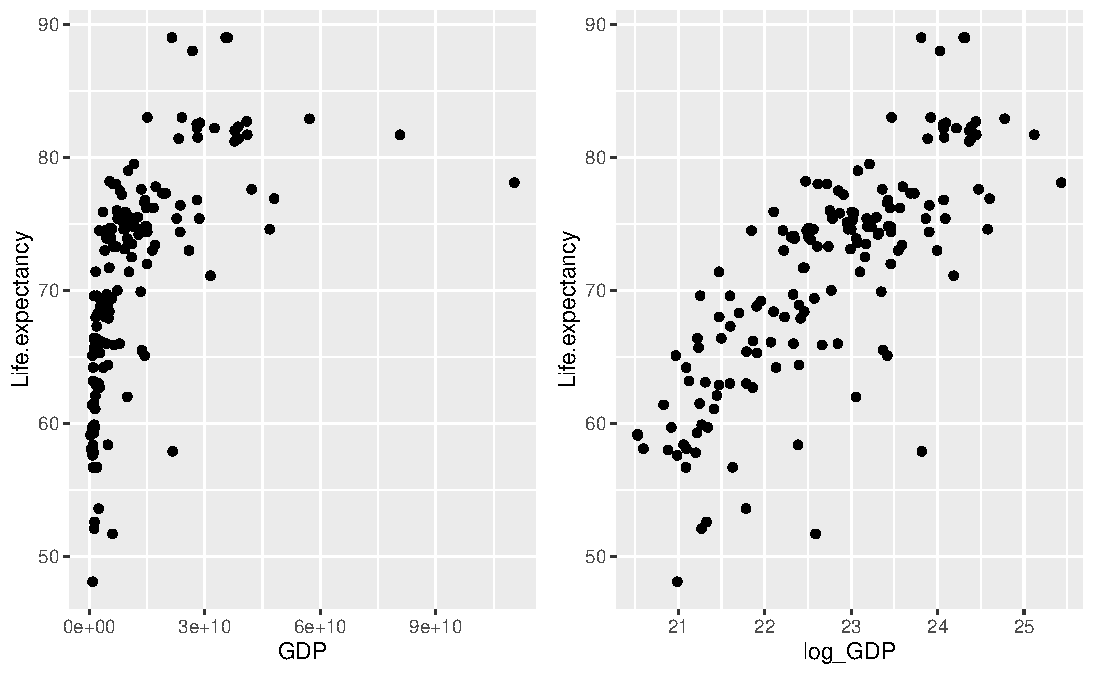
\includegraphics[width = 0.8\textwidth]{figures/transforms}
  \caption{Scatter plots of the GDP vs Life.expectancy variable before and after the transformation}
  \label{fig:transforms}
\end{figure}

In this subsection, the transformations applied to the dataset is described in detail. The GDP distribution before and after the log transformation is shown in figure \ref{fig:transforms}. The transformed function is created by the R code shown below:
\begin{verbatim}
transform <- function(x, scale) {
  if(scale == 0) return(log(1 + min(x) + x))
  else return(x^scale)
}
\end{verbatim}
The function takes two arguments, x as the original input value, and scale as the scaling value to be determined. A condition option for the user to choose when scale equals 0, the original input will be calculated as log(1 + min(x) + x); when the scale is given as a number that does not equal to 0, then the transformed input will be $x^{scale}$.



The transformations were applied as follows: log\_infant.deaths, log\_percentage.expenditure, log\_Measles, log\_under.five.deaths, log\_GDP, and log\_Population.

\begin{verbatim}
model2 <- lm(Life.expectancy ~ ., data = Dat2)
\end{verbatim}

The Adjusted R-squared: 0.8775, F-statistic: 59.83 and p-value: $< 2.2\times 10^{-16}$ was obtained from the new model on the new transformed dataset Dat2.

\subsection{Variance Inflation Factors}

The next step was to use the Variance Inflation Factors to check for multiple collinearity. This step was repeated several times to reduce multicollinearity from the model. The variable Hepatitis.B, log\_GDP, log\_Population, thinness.5.9.years, Income.composition.of.resources, and Schooling were removed. More details are provided in the evaluation section.


\begin{verbatim}
Dat3 <- Dat2[,-c(7, 15, 16, 18, 19, 20)]
model3 <- lm(Life.expectancy ~ ., data = Dat3)
\end{verbatim}
The new model showed the Adjusted R-squared: 0.7849, F-statistic:  44.8, and p-value: $< 2.2\times 10^{-16}$.


\subsection{Stepwise modeling}

The stepwise model selection approach is a way to iteratively add and/or remove candidate variables to build a subset of variables in the provided dataset for a better model. Stepwise regression includes forward, backward, and bidirectional methods. The bidirectional method was selected for this project for more flexible and appropriate models. The key R code to apply this step is listed below. Note the column "Status" is a binary categorical field, so it was converted the text values and assigned 1 for Developed and 0 for Developing.

\subsection{Bidirection model optimization}

\begin{verbatim}
DatSw <- Dat2
DatSw$Status <- ifelse(Dat$Status == "Developing", 0, 1)
stepwise(DatSw, "Life.expectancy", selection = "bidirection", select = "adjRsq")
\end{verbatim}

The library(StepReg), contains stepwise as a built-in function that provides the functionalities for the user to choose the direction to select the predictors, as well as the criterion. "adjRsq" as adjusted R squared is used to determine if the model improves with the addition or removal of a variable. During this step, variates "Adult.Mortality", "Alcohol", "log\_under.five.deaths", "HIV.AIDS","log\_percentage.expenditure", "Status", "Total.expenditure", "log\_infant.deaths", "Diphtheria", "BMI" and "thinness..1.19.years" were selected by the order of the improvement of "adjRsq".

\begin{verbatim}
DatSw <- select(Dat3_, c("Life.expectancy", sw$variate[-1]))
modelSw <- lm(Life.expectancy ~ ., data = DatSw)
\end{verbatim}

The model showed the Adjusted R-squared:  0.7876, F-statistic: 53.59 and p-value: $< 2.2\times 10^{-16}$. The adjusted R squared is expected to decrease since fewer variables were used in the current fitted model.

To optimize the model further, use of the vif function and methods to remove outliers were applied. Details will be provided separately in the Evaluation section. 

\subsection{Interactions}

% latex table generated in R 4.0.3 by xtable 1.8-4 package
% Thu Dec  9 18:45:49 2021
% latex table generated in R 4.0.3 by xtable 1.8-4 package
% Thu Dec  9 18:50:34 2021
% latex table generated in R 4.0.3 by xtable 1.8-4 package
% Thu Dec  9 18:51:17 2021
\begin{table}[ht]
\centering
\begin{tabular}{rlrr}
  \hline
 & v1v2 & $\Delta R^2$ & $\Delta adjR^2$ \\ 
  \hline
1 & Adult.Mortality*HIV.AIDS & 0.01650 & 0.01640 \\ 
  2 & Adult.Mortality*log\_under.five.deaths & 0.00680 & 0.00590 \\ 
  3 & Status*Diphtheria & 0.00680 & 0.00590 \\ 
  4 & Adult.Mortality*Total.expenditure & 0.00680 & 0.00580 \\ 
  5 & Adult.Mortality*log\_infant.deaths & 0.00660 & 0.00570 \\ 
   \hline
\end{tabular}
\caption{Effects of variable interaction} 
\label{tab:int}
\end{table}

Interactions were also a critical aspect to be considered. A simple R function, acting like a forward stepwise function, was written to probe all possible interactions between two variables and take the combination producing the largest increase for the adjusted R2 metric. In table \ref{tab:int} the best 5 best variants are shown and it is evident that  Adult.Mortality*HIV.AIDS should be used. As a result, the final model is defined as
\begin{verbatim}
final_model <- lm(Life.expectancy ~ 
   Alcohol + log_percentage.expenditure + Status + Total.expenditure 
   + Adult.Mortality*HIV.AIDS, data <- DatSw)
\end{verbatim}

An Adjusted R-squared of 0.804 was obtained with the added interaction in the model. After removing the variables that were not significant, an Adjusted R-squared of 0.7959, F-statistic: 87.89 and p-value: $< 2.2\times 10^{-16}$ were obtained. The last step to build the model is look for outliers and other high leverage points and will be explained in the Evaluation section separately.
% The final model we got is shown below with the Adjusted R-squared 0.7959, F-statistic 87.89, and the p-value $< 2.2\time 10^{-16}$. We are satisfied with this model as it gives a good Adjusted R-squared as well as a relatively acceptable number of predictors in the model.

% \begin{verbatim}
% model_cleaned <- lm(
%   Life.expectancy ~  Alcohol + log_percentage.expenditure + Status +
%    Total.expenditure + Adult.Mortality*HIV.AIDS
% , data = Dat_cleaned)
% \end{verbatim}

%%% Local Variables:
%%% TeX-master: "main"
%%% End:
